\documentclass[12pt]{beamer}
\usepackage[utf8]{inputenc}
%\usepackage[latin1]{inputenc}
\usepackage[spanish]{babel}
%\usetheme{Warsaw}
%\usepackage{euler}
\usepackage{amsmath}
\usepackage{amsthm}
\usepackage{booktabs}
\usepackage{tabulary}
\usepackage{nccmath}
\usepackage{multicol}
\usepackage{multirow}
\usepackage{graphicx}
\usepackage{tikz}
\usepackage{color}
\usepackage{listings}
\renewcommand*{\multirowsetup}{\centering}
\lstset{ %
language=Python,                % choose the language of the code
basicstyle=\small,       % the size of the fonts that are used for the code
numbers=left,                   % where to put the line-numbers
numberstyle=\footnotesize,      % the size of the fonts that are used for the line-numbers
stepnumber=1,                   % the step between two line-numbers. If it is 1 each line will be numbered
numbersep=5pt,                  % how far the line-numbers are from the code
backgroundcolor=\color{white},  % choose the background color. You must add \usepackage{color}
showspaces=false,               % show spaces adding particular underscores
showstringspaces=false,         % underline spaces within strings
showtabs=false,                 % show tabs within strings adding particular underscores
frame=single,   		% adds a frame around the code
tabsize=4,  		% sets default tabsize to 2 spaces
captionpos=b,   		% sets the caption-position to bottom
breaklines=true,    	% sets automatic line breaking
breakatwhitespace=false,    % sets if automatic breaks should only happen at whitespace
escapeinside={\#}{)}          % if you want to add a comment within your code
}
%\usepackage{epstopdf}
\DeclareGraphicsExtensions{.pdf,.png,.jpg}
\renewcommand {\arraystretch}{1.5}
\mode<presentation>
{
  \usetheme{Warsaw}
  \setbeamercovered{transparent}
  % or whatever (possibly just delete it)
}
\title{Tema 2 - Operaciones matem\'{a}ticas b\'{a}sicas}
\subtitle{C\'{a}lculo de ra\'{i}ces}
%\subsubtitle{Curso de F\'{i}sica Computacional}
\author{M. en C. Gustavo Contreras May\'{e}n}
%\date{18 de septiembre de 2012}
%\email{curso.fisica.comp@gmail.com}
%\ptsize{10}
\begin{document}
\maketitle
\fontsize{14}{14}\selectfont
\spanishdecimal{.}
\begin{frame}{Contenido}
\tableofcontents[pausesections]
\end{frame}
\section{C\'{a}lculo de ra\'{i}ces}
\begin{frame}
\frametitle{C\'{a}lculo de ra\'{i}ces}
Sea $y= f(x)$.  Los valores de $x$ que hacen que $y=0$ se
denominan \textcolor{blue}{ra\'{i}ces de la ecuaci\'{o}n}.
\\
\bigskip
El teorema fundamental del \'{a}lgebra indica que todo polinomio de grado $n$, tiene $n$ ra\'{i}ces. En el caso de las ra\'{i}ces reales, se tiene que corresponden a los valores $x$ que hacen que la funci\'{o}n corte el eje de las abscisas:
\end{frame}
\begin{frame}
\frametitle{Ejemplo de la funci\'{o}n seno(x)}
\begin{figure}
	\centering
	\includegraphics[scale=0.4]{raices00.eps} 
\end{figure}
\end{frame}
\begin{frame}
Las ra\'{i}ces de un polinomio pueden ser reales o complejas.
\\
\bigskip
Si un polinomio tiene coeficientes reales
\[ a_{0},a_{1},a_{2},\ldots,a_{n-1},a_{n} \]
entonces todas las ra\'{i}ces complejas siempre ocurrir\'{a}n en pares conjugados complejos.
\end{frame}
\begin{frame}
Por ejemplo, un polinomio c\'{u}bico tiene la siguiente
forma general:
\[ f(x)= a_{0}x^{3}+a_{1}x^{2}+a_{2}x+a_{3}\]
\begin{enumerate}
\item Tres ra\'{i}ces reales distintas.
\item Una ra\'{i}z real con multiplicidad 3.
\item Una ra\'{i}z real simple y una ra\'{i}z real con multiplicidad 2.
\item Una ra\'{i}z real y un par conjugado complejo.
\end{enumerate}
\end{frame}
\begin{frame}[fragile]
\frametitle{Tres ra\'{i}ces distintas}
\begin{minipage}{5cm}
\fontsize{12}{12}\selectfont
\[ \begin{split}
f(x)=& x^{3} - 3x^{2}-x+3 \\
=& (x-3)(x+1)(x-1)
\end{split} \]
Las ra\'{i}ces son:
\[ \begin{split}
x_{1} =& 3 \\
x_{2} =& -1 \\
x_{3} =& 1 \\
\end{split}\]
\end{minipage}
\hspace{0.5cm}
\begin{minipage}{4.5cm}
\begin{figure}
	\centering
	\includegraphics[scale=0.3]{raices01.eps} 
\end{figure}
\end{minipage}
\end{frame}
\begin{frame}[fragile]
\frametitle{Ra\'{i}z real con multiplicidad 3}
\begin{minipage}{5cm}
\fontsize{12}{12}\selectfont
\[ \begin{split}
f(x)=& x^{3} - 6x^{2} + 12x - 8 \\
=& (x-2)^{3}
\end{split} \]
Las ra\'{i}ces son:
\[ \begin{split}
x_{1} =& 2 \\
x_{2} =& 2 \\
x_{3} =& 2 \\
\end{split}\]
\end{minipage}
\hspace{0.5cm}
\begin{minipage}{4.5cm}
\begin{figure}
	\centering
	\includegraphics[scale=0.3]{raices02.eps} 
\end{figure}
\end{minipage}
\end{frame}
\begin{frame}[fragile]
\frametitle{Ra\'{i}z real simple y \\ una ra\'{i}z real con multiplicidad 2}
\begin{minipage}{5cm}
\fontsize{12}{12}\selectfont
\[ \begin{split}
f(x)=& x^{3} - 12x + 16 \\
=& (x+4)(x-2)^{2}
\end{split} \]
Las ra\'{i}ces son:
\[ \begin{split}
x_{1} =& -4 \\
x_{2} =& 2 \\
x_{3} =& 2 \\
\end{split}\]
\end{minipage}
\hspace{0.5cm}
\begin{minipage}{4.5cm}
\begin{figure}
	\centering
	\includegraphics[scale=0.3]{raices03.eps} 
\end{figure}
\end{minipage}
\end{frame}
\begin{frame}[fragile]
\frametitle{Ra\'{i}z real y un par conjugado complejo}
\begin{minipage}{5cm}
\fontsize{12}{12}\selectfont
\[ \begin{split}
f(x)=& x^{3} - 2x^{2}- 3x +10  \\
=& (x+2)(x- (2+i))* {}\\
*& (x-(2-i))
\end{split} \]
Las ra\'{i}ces son:
\[ \begin{split}
x_{1} =& -2 \\
x_{2} =& 2+i \\
x_{3} =& 2-i \\
\end{split}\]
\end{minipage}
\hspace{0.5cm}
\begin{minipage}{4.5cm}
\begin{figure}
	\centering
	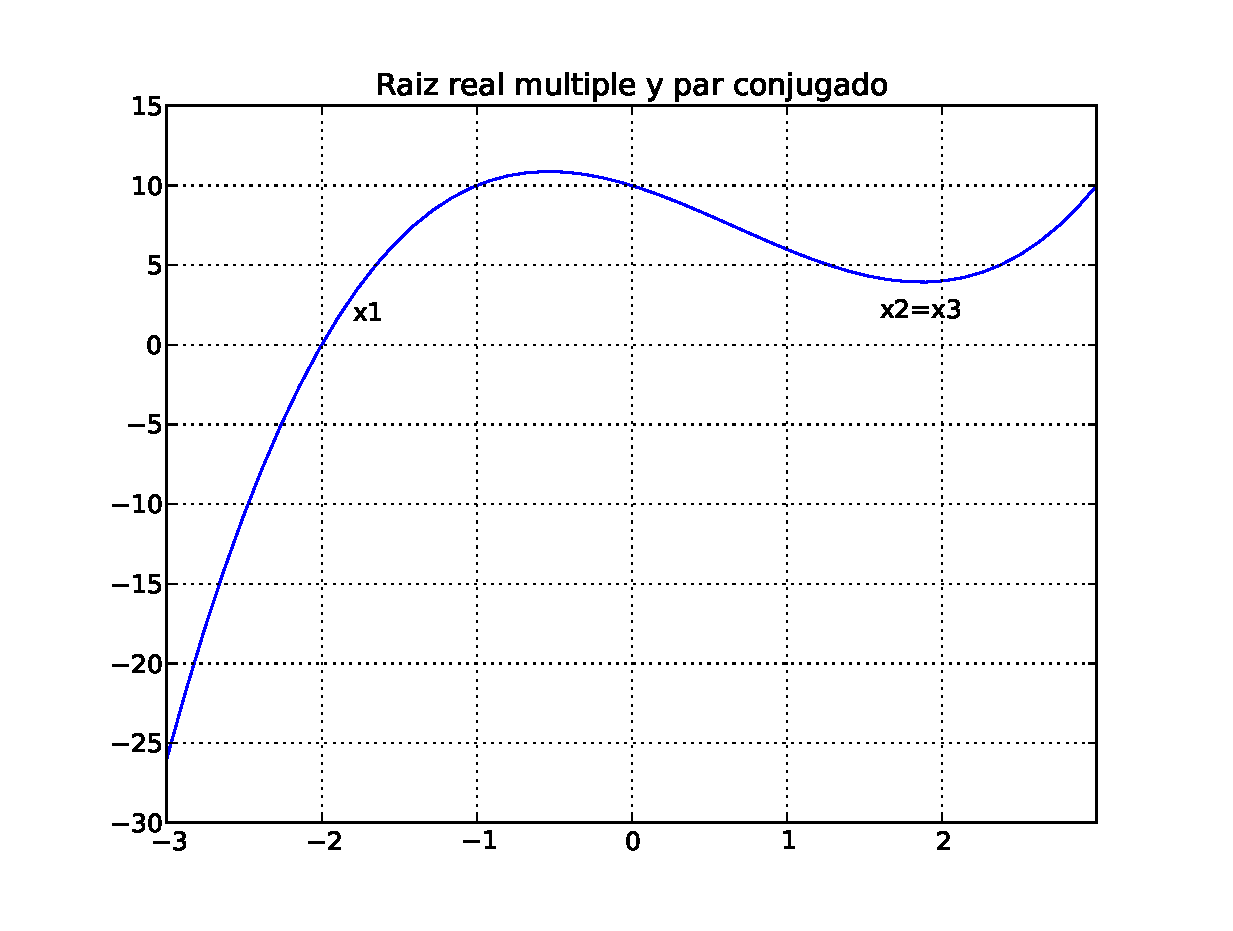
\includegraphics[scale=0.3]{raices04.eps} 
\end{figure}
\end{minipage}
\end{frame}
\section{Funciones algebraicas}
\begin{frame}
\frametitle{Funciones algebraicas}
Sea $g=f(x)$ la funci\'{o}n expresada como
\[ f_{n}y^{n} + f_{n-1}y^{n-1} + \ldots + f_{1}y + f_{0} = 0 \]
Donde $f_{i}$ es un polinomio de orden $i$ en $x$.
\\
\bigskip
Los polinomios son un caso simple de funciones algebraicas que se representan generalmente como
\[f_{n}(x) = a_{0} + a_{1}x + a_{2} x^{2}+ \ldots +a_{n}x^{n} \]
Donde $n$ es el orden del polinomio.
\end{frame}
\section{Funciones trascendentales}
\begin{frame}
\frametitle{Funciones trascedentales}
Son aquellas que no son algebraicas.
\\
\bigskip
Comprenden a las funciones trigonom\'{e}tricas, exponenciales, logar\'{i}tmicas, entre otras.
\\
\bigskip
Ejemplos:
\begin{itemize}
\item \[ f(x)=ln(x^{2}-1) \]
\item \[g(x)=e^{-0.2x} \sin(3x-5) \]
\end{itemize}
\end{frame}
\begin{frame}
Los m\'{e}todos num\'{e}ricos est\'{a}ndar para encontrar
ra\'{i}ces pueden clasificarse en dos rubros:
\\
\bigskip
\textbf{1.} La determinaci\'{o}n de las ra\'{i}ces reales de ecuaciones algebraicas y trascendentales. Las t\'{e}cnicas a emplear en estos casos se diseñaron con el fin de encontrar el valor de una ra\'{i}z simple de acuerdo con un conocimiento previo de su posici\'{o}n aproximada.
\end{frame}
\begin{frame}
\textbf{2.} La determinaci\'{o}n de todas las raíces reales y complejas de un polinomio, para lo cual los m\'{e}todos num\'{e}ricos est\'{e}n diseñados espec\'{i}ficamente para polinomios. 
\\
\bigskip
Determinan sistem\'{a}ticamente todas las ra\'{i}ces del polinomio en lugar de hacerlo s\'{o}lo con una, dada la posición aproximada.
\end{frame}
\section{M\'{e}todo de incrementos sucesivos}
\begin{frame}
\frametitle{M\'{e}todo de incrementos sucesivos}
Podemos aproximar mucho mejor las ra\'{i}ces de una funci\'{o}n, cuando la graficamos.
\\
\bigskip
Con una gr\'{a}fica general de unos cuantos puntos, tendr\'{i}amos lo necesario para considerar los valores de las ra\'{i}ces.
\\
\bigskip
El m\'{e}todo de b\'{u}squeda incremental es una herramienta \'{u}til que podemos adoptar en conjunto con otras estrategias de c\'{a}lculo de ra\'{i}ces, por s\'{i} s\'{o}lo, \'{e}ste m\'{e}todo no nos ofrece m\'{a}s que una referencia sobre en d\'{o}nde podr\'{i}an estar esas ra\'{i}ces.
\end{frame}
\begin{frame}
La idea b\'{a}sica detr\'{a}s del m\'{e}todo de b\'{u}squeda incremental es simple: si $f(x_{1})$ y $f(x_{2})$ tienen signos opuestos, entonces hay al menos una ra\'{i}z en el intervalo $(x_{1}, x_{2})$.
\end{frame}
\begin{frame}[fragile]
\frametitle{Caso en donde es posible encontrar la ra\'{i}z}
\begin{center}
	\begin{tikzpicture}[font=\footnotesize, scale=1.3]
		\draw[<->](0,0) -- (6,0);
		\draw[<->](3,-2) -- (3,2);
		\draw [red] (0.5,1.5) .. controls (2,0.2) and (4,-1) .. (5.5,-1.5);
		\draw[dashed] (1,0) -- (1,1.1);
		\draw (0.9,-0.2) node {a}; 
		\draw (1.2,1.4) node {f(a)};
		\draw[dashed] (5,0) -- (5,-1.33);
		\draw (5,0.2) node {b}; 
		\draw (5,-1.7) node {f(b)};
		\draw(4.5,1.5) node {$f(a)*f(b)<0$};
	\end{tikzpicture}
\end{center}
\end{frame}
\begin{frame}
\frametitle{Caso en donde no es posible encontrar la ra\'{i}z}
\begin{center}
	\begin{tikzpicture}[font=\footnotesize, scale=1.3]
		\draw[<->](0,0) -- (6,0);
		\draw[<->](3,-1) -- (3,3);
		\draw [red] (0.5,2.5) .. controls (2.5,0.5) and (3.5,0.5) .. (5.5,2.5);
		\draw [dashed] (1,0) -- (1,2.1);
		\draw (1,-0.2) node {a};
		\draw (1.1,2.2) node {f(a)};
		\draw [dashed] (4.5,0) -- (4.5,1.65);
		\draw (4.5,-0.2) node {b};
		\draw (4.5, 2) node {f(b)};
		\draw (5,3.5) node {$f(a)*f(b)>0$};
	\end{tikzpicture}
\end{center}
\end{frame}
\begin{frame}
Si el intervalo es lo suficientemente pequeño, es probable que contenga una sola ra\'{i}z. As\'{i}, los ceros de $f(x)$ puede ser detectados mediante la evaluaci\'{o}n de la funci\'{o}n a intervalos $\Delta x$ y mirando cuando se presente un cambio de signo en la funci\'{o}n.
\end{frame}
\begin{frame}
Hay varios problemas con el m\'{e}todo de b\'{u}squeda incremental:
\begin{enumerate}
\item Es posible perder dos ra\'{i}ces muy pr\'{o}ximas entre s\'{i}, si el incremento de búsqueda $\Delta x$ es mayor que la separaci\'{o}n de las ra\'{i}ces.
\item Una ra\'{i}z doble (dos ra\'{i}ces que coinciden) no ser\'{a} detectada.
\item Algunas singularidades de $f(x)$ se puede confundir con ra\'{i}ces. Por ejemplo, $f(x) = \tan x$. Tiene cambios de signo en $x = \pm 1/2 n\pi$ con $n = 1, 3, 5,\ldots$
\end{enumerate}
\end{frame}
\begin{frame}
Estos puntos no son ceros verdaderos, ya que la funci\'{o}n no cruza el eje $x$.
\begin{figure}
	\centering
	\includegraphics[scale=0.4]{raices05.eps} 
\end{figure}
\end{frame}
\subsection{C\'{o}digo M\'{e}todo de incrementos sucesivos}
\begin{frame}
\frametitle{C\'{o}digo M\'{e}todo de incrementos sucesivos}
El c\'{o}digo busca un cero de la función $f$ que proporciona el usuario en el intervalo
$(a,b)$ en incrementos de $dx$.
\\
\bigskip
Se devuelve el intervalo $(x_{1}, x_{2})$ donde se encuentra la ra\'{i}z, si la b\'{u}squeda
se ha realizado correctamente; se devuelve $x_{1} = x_{2} = \mathsf{None}$ cuando no se encontraron ra\'{i}ces.
\\
\bigskip
Luego de que se encontr\'{o} la primera ra\'{i}z, (la m\'{a}s cercana al punto $a$), se puede llamar de nuevo al procedimiento, sustitiyendo $x_{2}$ con el fin de encontrar la siguiente ra\'{i}z. Esto se puede repetir siempre y cuando se detecta una ra\'{i}z.
\end{frame}
\begin{frame}[fragile]
\begin{lstlisting}
def buscaraiz(f,a,b,dx):
    x1 = a; f1 = f(a)
    x2 = a + dx; f2 = f(x2)
    while f1*f2 > 0.0:
        if x1 >= b: return None
        x1 = x2; f1 = f2
        x2 = x1 + dx; f2 = f(x2)
    else:
        return x1,x2
\end{lstlisting}
\end{frame}
\begin{frame}
\frametitle{Ejemplo}
Usa el m\'{e}todo de incrementos sucesivos y con $\Delta x= 0.2$, para estimar la ra\'{i}z con el valor positivo m\'{a}s pequeño de la funci\'{o}n:
\[ f(x) = x^{3} - 10 x^{2} + 5\]
\end{frame}
\begin{frame}
\begin{figure}
	\centering
	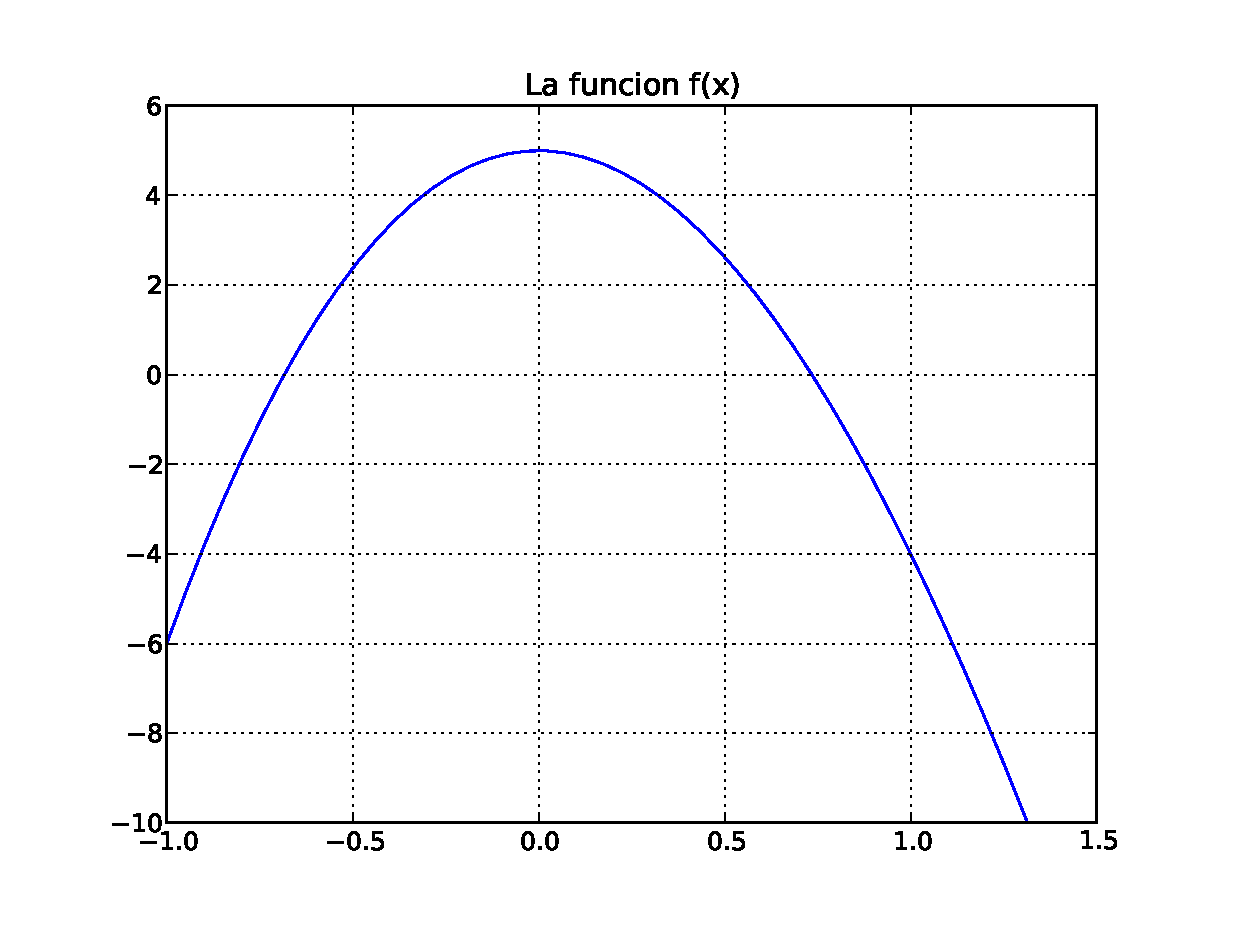
\includegraphics[scale=0.5]{raices06.eps} 
\end{figure}
\end{frame}
\begin{frame}[fragile]
\begin{lstlisting}
def f(x): return x**3 - 10*x**2 + 5.

a, b, dx = (0.0,1.5, 0.2)

print 'El intervalo es: '
x1, x2 = buscaraiz(f,a,b,dx)
print x1,x2
\end{lstlisting}
\end{frame}
\section{M\'{e}todo de Bisecci\'{o}n}
\begin{frame}
\frametitle{{M\'{e}todo de Bisecci\'{o}n}}
Despu\'{e}s de que se ha identificado una ra\'{i}z $f(x) = 0$ en el intervalo $(x_{1}, x_{2})$, disponemos de varios m\'{e}todos para encontrar el valor de la ra\'{i}z.
\\
\bigskip
El m\'{e}todo de bisecci\'{o}n logra esta tarea: \textcolor{red}{el intervalo se reduce sucesivamente a la mitad  hasta que se vuelve suficientemente pequeño}. La t\'{e}cnica de bisecci\'{o}n no es el m\'{e}todo m\'{a}s r\'{a}pido disponible, pero es el m\'{a}s fiable. Una vez que una raíz se ha encontrado en un intervalo, nos podemos acercar a ella.
\end{frame}
\begin{frame}
El m\'{e}todo de bisecci\'{o}n utiliza el mismo principio que el incremento sucesivo: si hay una ra\'{i}z en el intervalo $(x_{1}, x_{2})$, entonces $f(x_{1})*f(x_{2})<0$.
\end{frame}
\begin{frame}
Con el fin de reducir a la mitad el intervalo, se calcula $f(x_{3})$, donde $x_{3} = (x1 + x2)/2$ es el punto medio del intervalo.
\end{frame}
\begin{frame}
\setbeamercovered{invisible}
\begin{center}
	 \begin{tikzpicture}[font=\footnotesize, scale=1.3]
		\draw[->](0,0) -- (6,0);
		\draw[<->](0,-2) -- (0,2);
		\draw [red] (0.5,1.5) .. controls (2,0.2) and (4,-1) .. (5.5,-1.5);
		\draw[dashed] (1,0) -- (1,1.1);
		\draw (0.9,-0.2) node {$x_{1}$};
		\draw (0.9,1.5) node {$f(x_{1})$}; 
		\draw[dashed] (5,0) -- (5,-1.33);
		\draw (5,0.2) node {$x_{2}$};
		\draw (5,-1.6) node {$f(x_{2})$};\pause
		\draw (3,0.2) node {$x_{3}$};\pause
		\draw [dashed] (3,0) -- (3,-0.3);
		\draw (3,-0.7) node {$f(x_{3})$};
	\end{tikzpicture}
\end{center}
\end{frame}
\begin{frame}
Si $f(x_{1})*f(x_{3}) < 0$, entonces la ra\'{i}z debe estar en $(x_{1}, x_{3})$ entonces re-emplazamos del intervalo inicial $x_{2}$ por $x_{3}$. De lo contrario, la ra\'{i}z se encuentra en $(x_{3}, x_{2})$, en tal caso, se sustituye $x_{3}$ por $x_{1}$.
\setbeamercovered{invisible}
\pause
\begin{center}
	 \begin{tikzpicture}[font=\footnotesize]
		\draw[->](0,0) -- (6,0);
		\draw[<->](0,-2) -- (0,2);
		\draw [red] (0.5,1.5) .. controls (2,0.2) and (4,-1) .. (5.5,-1.5);
		\draw[dashed] (1,0) -- (1,1.1);
		\draw (0.9,-0.2) node {$x_{1}$};
		\draw (0.9,1.5) node {$f(x_{1})$}; 
		\draw (3,0.2) node {$x_{2}$};
		\draw [dashed] (3,0) -- (3,-0.3);
		\draw (3,-0.7) node {$f(x_{2})$};\pause
		\draw (2,-0.2) node {$x_{3}$};
		\draw [dashed] (2,0) -- (2,0.3);
		\draw (2,0.7) node {$f(x_{3})$};
	\end{tikzpicture}
\end{center}
\end{frame}
\begin{frame}
En cualquiera de los casos, el nuevo intervalo $(x_{1}, x_{2})$ es la mitad del tamaño del intervalo original. La bisecci\'{o}n es repite hasta que el intervalo se ha reducido a un valor $\epsilon$ pequeño, de modo que
\[ \vert x_{2} - x_{1} \vert \leq \epsilon\]
\end{frame}
\begin{frame}
Es f\'{a}cil calcular el n\'{u}mero de bisecciones necesarias para alcanzar el valor de $\epsilon$. El intervalo inicial $\Delta x$, se reduce a $\Delta x /2$ en la primera bisecci\'{o}n, $\Delta x /2^{2}$ en la segunda, luego de $n$ bisecciones, $\Delta x /2^{n}$. Haciendo $\Delta x /2^{n} = \epsilon$, resolvemos para $n$
\[ n = \dfrac{ln(\vert \Delta x \vert/ \epsilon)}{ln 2}\]
\end{frame}
\begin{frame}
Implementa el m\'{e}todo de bisecci\'{o}n para calcular la(s) ra\'{i}z(ces) de:
\begin{enumerate}
	\item \[ x^{3} - 10^{2} + 5\]
	\item \[  x- \tan(x) \hspace{1cm} 0 \leq x \leq 20\]
\end{enumerate}
Con una tolerancia de $1\times 10^{-4}$
\end{frame}
\end{document}